\documentclass[8pt,a4paper,compress]{beamer}

\usepackage{/home/siyer/lib/slides}

\title{Basic Programming Model}
\date{}

\begin{document}
\begin{frame}
\vfill
\titlepage
\end{frame}

\begin{frame}
\frametitle{Outline}
\tableofcontents
\end{frame}

\section{Basic Structure of a Java Program}

\begin{frame}[fragile]
\begin{itemize}
\item the Java workflow

\smallskip

\begin{center}
\begin{tikzpicture}
\begin{scope}[->,xshift=-7.5cm,yshift=-5cm,thin,
	   node distance=1.6cm,on grid,>=stealth,
  	   block1/.style={rectangle,draw,align=center},
	   block2/.style={rectangle,align=center}]
\node [block1] (1) {editor \\ (BlueJ)};
\node [block2] (2) [right=of 1] {\lstinline$P.java$};
\node [block1] (3) [right=of 2] {compiler \\ (\lstinline$javac$)};
\node [block2] (4) [right=of 3] {\lstinline$P.class$};
\node [block1] (5) [right=of 4] {JVM \\ (\lstinline$java$)};
\node [block2] (6) [right=of 5] {output};
\path (1) edge node [above] {} (2);
\path (2) edge node [above] {} (3);
\path (3) edge node [above] {} (4);
\path (4) edge node [above] {} (5);
\path (5) edge node [above] {} (6);
\end{scope}
\end{tikzpicture}
\end{center}

\item a Java program is either a library of static methods (functions) or a data type definition

\item to create a Java program (class), we use the following programming constructs

\begin{itemize}
\item primitive data types and expressions

\item statements

\item arrays

\item static methods

\item strings

\item input and output (IO)

\item data abstraction
\end{itemize}
\end{itemize}
\end{frame}

\begin{frame}[fragile]
\begin{itemize}
\item prime counter

\begin{lstlisting}[language=Java]
public class PrimeCounter {
    public static boolean isPrime(int N) {
        if (N < 2) {
            return false;
        }
        for (int i = 2; i <= N / i; i++) {
            if (N % i == 0) {
                return false;
            }
        }
        return true;
    }

    public static int countPrimes(int N) {
        int count = 0;
        for (int i = 2; i <= N; i++) {
            count += isPrime(i) ? 1 : 0;
        }
        return count;
    }
    
    public static void main(String[] args) {
        int N = Integer.parseInt(args[0]);
        StdOut.println("Number of primes <= " + N + " is " 
                       + countPrimes(N));
    }
}
\end{lstlisting}

\begin{lstlisting}[language={}]
$ javac PrimeCounter.java
$ java PrimeCounter 1000
Number of primes <= 1000 is 168
\end{lstlisting}
\end{itemize}
\end{frame}

\section{Primitive Data Types and Expressions}

\begin{frame}[fragile]
\begin{itemize}
\item a data type (primitive or reference) is a set of values and a set of operations on those values

\item basic primitive types
\begin{itemize}
\item \lstinline{boolean}: true and false values with logical operations (\lstinline{!}, \lstinline{||}, and \lstinline{&&})
\item \lstinline{char}: 16-bit characters with arithmetic operations (\lstinline{+}, \lstinline{-}, \lstinline{*}, \lstinline{/}, and \lstinline{%})
\item \lstinline{int}: 32-bit integers with arithmetic operations
\item \lstinline{double}: 64-bit double-precision real numbers with arithmetic operations
\end{itemize}

\item other primitive types
\begin{itemize}
\item \lstinline{byte}: 8-bit integers with arithmetic operations
\item \lstinline{short}: 16-bit integers with arithmetic operations
\item \lstinline{float}: 32-bit single-precision real numbers with arithmetic operations
\item \lstinline{long}: 64-bit integers with arithmetic operations
\end{itemize}
\end{itemize}
\end{frame}

\begin{frame}[fragile]
\begin{itemize}
\item an expression is a literal, a variable, or a sequence of allowed operations on literals and/or variables that produces a value

\item arithmetic operators \lstinline{*} and \lstinline{/} have higher precedence than \lstinline{+} and \lstinline{-}

\item among logical operators, \lstinline{!} has the highest precedence, followed by \lstinline{&&} and then \lstinline{||}

\item two operands of the same type can be compared using the relational operators \lstinline{==}, \lstinline{!=}, \lstinline{<}, \lstinline{<=}, \lstinline{>}, and \lstinline{>=}, producing a Boolean result

\item relational operators have higher precedence than logical operators but lower precedence than arithmetic operators

\item operators of the same precedence are evaluated left to right

\item parentheses can be used to override precedence rules

\item numbers are automatically promoted to a more inclusive type if no information is lost

\item a cast is a type name in parentheses within an expression, and converts the following value into a value of that type
\end{itemize}
\end{frame}

\section{Statements}
\begin{frame}[fragile]
\begin{itemize}
\item a statement defines computation by creating variables, assigning data-type values to them, and controlling the flow of execution

\item a declaration statement associates a variable name with a type
\begin{lstlisting}[language={}]
<type> <name>;
\end{lstlisting}
where the initial value for the variable is \lstinline{false} for Boolean type, \lstinline{0} for numeric types, and \lstinline{null} for reference types

\item an assignment statement associates a data-type value with a variable
\begin{lstlisting}[language={}]
<name> = <expression>;
\end{lstlisting}

\item declaration and assignment statements can be combined to provide an initial value for a variable
\begin{lstlisting}[language={}]
<type> <name> = <expression>;
\end{lstlisting}
\end{itemize}
\end{frame}

\begin{frame}[fragile]
\begin{itemize}
\item a conditional statement is used when different actions are required for different inputs

\begin{itemize}
\item if statement
\begin{lstlisting}[language={}]
if (<boolean expression>) {
    <statements>
}
else if (<boolean expression>) {
    <statements>
}
...
else {
    <statements>
}
\end{lstlisting}

\item conditional operator (really an expression)
\begin{lstlisting}[language={}]
<boolean expression> ? <expression> : <expression>
\end{lstlisting}

\item switch statement 
\begin{lstlisting}[language={}]
switch (<expression>) {
    case <value>:
        <statements>
    case <value>:
        <statements>
    ...
    default:
        <statements>
}
\end{lstlisting}

\end{itemize}
 
\end{itemize}
\end{frame}

\begin{frame}[fragile]

\begin{itemize}
\item a loop statement is used for repetitive computations

\begin{itemize}
\item while statement
\begin{lstlisting}[language={}]
while (<boolean expression>) {
    <statements>
}
\end{lstlisting}

\item for statement
\begin{lstlisting}[language={}]
for (<initialize>; <boolean expression>; <increment>) {
    <statements>
}
\end{lstlisting}

\item do-while statement 
\begin{lstlisting}[language={}]
do {
    <statements>
} while (<boolean expression>);
\end{lstlisting}

\item a break statement immediately exits a loop without letting it to run to completion

\item a continue statement skips to next iteration of a loop
\end{itemize}

\item a compound assignment statement is shorthand notation for modifying the value of a variable

\item the scope of a variable is the statements that follow the declaration in the same block (marked by curly brackets) as the declaration
\end{itemize}
\end{frame}

\section{Arrays}
\begin{frame}[fragile]
\begin{itemize}
\item an array stores a sequence of values that are all of the same type 

\item making an array in Java involves: declaring the array name and type; creating the array; and initializing the array values
\begin{lstlisting}[language=Java]
int[] a;
a = new int[10];
for (int i = 0; i < 10; i++) {
    a[i] = i;
}
\end{lstlisting}

\item an array when declared is initialized to \lstinline{null}, and once created, each element is initialized to a default value based on the type of the array

\item initializing declaration
\begin{lstlisting}[language=Java]
int[] a = {1, 1, 2, 3, 5, 8, 13, 21, 34, 55};
String[] b = {"Sun", "Mon", "Tue", "Wed", "Thu", "Fri", "Sat"};
\end{lstlisting}

\item reversing an array in place
\begin{lstlisting}[language=Java]
int N = a.length;
for (int i = 0; i < N / 2; i++) {
    double temp = a[i];
    a[i] = a[N - 1 -i];
    a[N - i - 1] = temp;
}
\end{lstlisting}

\end{itemize}
\end{frame}

\begin{frame}[fragile]
\begin{itemize}
\item if we assign one array name to another (aliasing), then both refer to the same array

\item a two-dimensional array in Java is an array of one-dimensional arrays

\item a two-dimensional array may be ragged

\item initializing declaration for two-dimensional arrays
\begin{lstlisting}[language=Java]
int[][] I = {{1, 0, 0}, 
              0, 1, 0}, 
              0, 0, 1}};
\end{lstlisting}

\item matrix multiplication $$C_{ij}=\sum_{k=1}^{p} A_{ik}B_{kj},$$ where $A$ is an $m\times p$, $B$ is a $p \times n$, and $C$ is an $m\times n$ matrix
\begin{lstlisting}[language=Java]
int m = A.length;
int p = B.length;
int n = B[0].length;
double[][] C = new double[m][n];
for (int i = 0; i < m; i++) {
    for (int j = 0; j < n; j++) {
        for (int k = 0; k < p; k++) {
            C[i][j] += A[i][k] * B[k][j];
        }
    }
}
\end{lstlisting}

\end{itemize}
\end{frame}

\section{Static Methods}
\begin{frame}[fragile]
\begin{itemize}
\item a method encapsulates a computation defined as a sequence of statements

\item a static method is composed of the keywords \lstinline{public static} followed by a return type (or \lstinline{void}), the signature (method name and a sequence of arguments, each with a declared type), and a body (a sequence of statements enclosed by curly brackets)

\item primality testing
\begin{lstlisting}[language=Java]
public static boolean isPrime(int N) {
    if (N < 2) {
        return false;
    }
    for (int i = 2; i <= N / i; i++) {
        if (N % i == 0) {
            return false;
        }
    }
    return true;
}
\end{lstlisting}

\item a call on a static method is its name followed by expressions that specify argument values in parentheses, separated by commas

\item when a method call is part of an expression, the method computes a value and that value is used in place of the call in the expression

\item a method call followed by a semicolon is a statement that generally causes side effects
\end{itemize}
\end{frame}

\begin{frame}[fragile]
\begin{itemize}
\item properties of methods
\begin{itemize}
\item arguments are passed by value
\item method names can be overloaded 
\item a method has a single return value but may have multiple return statements
\item a method can have side effects
\end{itemize}

\item a recursive method is one that calls itself, has a base case, addresses subproblems that are smaller in some sense, and does not address subproblems that overlap

\item computing $N!$ (good recursion)
\begin{lstlisting}[language=Java]
public static int factorial(int N) {
    return (N == 0) ? 1 : N * factorial(N - 1); 
}
\end{lstlisting}

\item computing $N$th Fibonacci number (bad recursion)
\begin{lstlisting}[language=Java]
public static int fibonacci(int N) {
    return (N == 0 || N == 1) ? 1 : fibonacci(N - 1) + fibonacci(N - 2); 
}
\end{lstlisting}
\end{itemize}
\end{frame}

\begin{frame}[fragile]
\begin{itemize}
\item a best practice in Java programming is to include a \lstinline{main()} method (aka development or test client) in every library of static methods

\item we use static methods from four different kinds of libraries
\begin{itemize}
\item standard system libraries \lstinline{java.lang.*}
\item imported system libraries such as \lstinline{java.util.Arrays}
\item other libraries in the text
\item standard libraries \lstinline{Std*} from the text
\end{itemize}
\end{itemize}
\end{frame}

\section{APIs}
\begin{frame}[fragile]
\begin{itemize}
\item an application programming interface (API) lists the library name and the return type, signatures, and short descriptions of each of the methods

\item a client is a program that calls a method in another library

\item an implementation is a Java code that implements the methods in an API

\item consider every program that you write as a library implementation, for possible reuse in the future

\item Java libraries
\begin{itemize}
\item \lstinline{java.lang.Math}
\begin{lstlisting}[language={},mathescape]
public class Math

    double abs(double a)           // $|a|$
    double max(double a, double b) // $\max(a, b)$
    double min(double a, double b) // $\min(a, b)$
    double sin(double theta)       // $\sin(\theta)$
    double cos(double theta)       // $\cos(\theta)$
    double tan(double theta)       // $\tan(\theta)$
    double random()                // $\text{real} \in [0, 1)$
    double E                       // $e$
    double PI                      // $\pi$
    ...
\end{lstlisting}

\item \lstinline{java.util.Arrays}
\begin{lstlisting}[language={}]
public class Arrays

    void sort(int[] a) // put the array in ascending order
    ...
\end{lstlisting}
\end{itemize}
\end{itemize}
\end{frame}

\begin{frame}[fragile]
\begin{itemize}
\item standard libraries from the text
\begin{itemize}
\item \lstinline{StdRandom}
\begin{lstlisting}[language={},mathescape]
public class StdRandom

    void initialize(long seed)           // initialize
    double random()                      // $\text{real} \in [0, 1)$
    int uniform(int N)                   // $\text{integer} \in [0, N)$
    int uniform(int lo, int hi)          // $\text{integer} \in [lo, hi)$
    double uniform(double lo, double hi) // $\text{real} \in [lo, hi)$
    boolean bernoulli(double p)          // true with probability $p$
    double gaussian()                    // $\text{real} \in \mathcal{N}(0, 1)$
    double gaussian(double m, double s)  // $\text{real} \in \mathcal{N}(m, s)$
    int discrete(double[] a)             // $i$ with probability $a[i]$
    void shuffle(double[] a)             // shuffle the array
    ...
\end{lstlisting}

\item \lstinline{StdStats}
\begin{lstlisting}[language={}]
public class StdStats

    double max(double[] a)    // largest value
    double min(double[] a)    // smallest value
    double mean(double[] a)   // average
    double var(double[] a)    // sample variance
    double stddev(double[] a) // sample standard deviation
    double median(double[] a) // median
    ...
\end{lstlisting}
\end{itemize}
\end{itemize}
\end{frame}

\section{Strings}
\begin{frame}[fragile]
\begin{itemize}
\item a string is a sequence of characters (\lstinline{char} values) 

\item a string literal is a sequence of characters within double quotes, such as \lstinline{"Hello, World"}

\item the result of concatenating two strings using the \lstinline{+} operator is a single string, the first string followed by the second

\item we use Java library methods such as \lstinline{Integer.parseInt()}, \lstinline{Double.parseDouble()}, and so on to convert strings to primitives

\item we use the \lstinline{+} operator to convert primitives to strings
\end{itemize}
\end{frame}

\section{Input and Output}
\begin{frame}[fragile]
\begin{itemize}
\item bird's-eye biew of a Java program
\begin{center}
\begin{tikzpicture}
\begin{scope}[->,xshift=-7.5cm,yshift=-5cm,thin,
	   node distance=1.6cm,on grid,>=stealth,
  	   block1/.style={rectangle,draw,align=center},
	   block2/.style={rectangle,align=center}]
\node [block2] (1) {input};
\node [block1] (2) [right=of 1] {\lstinline{P.java}};
\node [block2] (3) [right=of 2] {output};
\path (1) edge node [above] {} (2);
\path (2) edge node [above] {} (3);
\end{scope}
\end{tikzpicture}
\end{center}

\begin{itemize}
\item input types: command-line arguments, standard input, file input
\item output types: standard output, file output, graphical output
\end{itemize}

\item \lstinline{StdOut}
\begin{lstlisting}[language={},mathescape]
public class StdOut

    void print(String s)       // print $s$
    void println(String s)     // print $s$, followed by a newline
    void println()             // print a newline
    void printf(String f, ...) // formatted print
    ...
\end{lstlisting}

\item \lstinline{StdOut} client
\begin{lstlisting}[language=Java]
public class RandomSeq {
    public static void main(String[] args) { 
        int N = Integer.parseInt(args[0]);
        double lo = Double.parseDouble(args[1]);
        double hi = Double.parseDouble(args[2]);
        for (int i = 0; i < N; i++) {
            double x = StdRandom.uniform(lo, hi);
            StdOut.printf("%.2f\n", x);
        }
    }
}
\end{lstlisting}

\begin{lstlisting}[language={}]
$ java RandomSeq 2 100.0 200.0
193.12
190.79
\end{lstlisting}
\end{itemize}
\end{frame}

\begin{frame}[fragile]
\begin{itemize}
\item \lstinline{StdIn}
\begin{lstlisting}[language={},mathescape]
public class StdIn

    boolean isEmpty()     // true if no more values, false otherwise
    int readInt()         // read a value of type int
    double readDouble()   // read a value of type double
    boolean readBoolean() // read a value of type boolean
    char readChar()       // read a value of type char
    String readString()   // read a value of type String
    boolean hasNextLine() // is there another line in the input stream?
    String readLine()     // read the rest of the line
    String readAll()      // read the rest of the input stream
    ...
\end{lstlisting}

\item \lstinline{StdIn} client
\begin{lstlisting}[language=Java]
public class Average { 
    public static void main(String[] args) { 
        int count = 0; 
        double sum = 0.0;
        while (!StdIn.isEmpty()) {
            double value = StdIn.readDouble();
            sum += value;
            count++;
        }
        double average = sum / count;
        StdOut.println("Average is " + average);
    }
}
\end{lstlisting}

\begin{lstlisting}[language={}]
$ java Average
1 2 3 4 5
<ctrl-d>
Average is 3.0
\end{lstlisting}

\end{itemize}
\end{frame}

\begin{frame}[fragile]
\begin{itemize}
\item redirection and piping
\begin{lstlisting}[language={}]
$ java RandomSeq 1000 100.0 200.0 > data.txt
$ head -5 data.txt
155.83
191.65
197.83
191.90
111.84
\end{lstlisting}

\begin{lstlisting}[language={}]
$ java Average < data.txt
Average is 149.1812199999999
\end{lstlisting}

\begin{lstlisting}[language={}]
$ java RandomSeq 1000 100.0 200.0 | java Average
Average is 150.0588699999999
\end{lstlisting}
\end{itemize}
\end{frame}

\begin{frame}[fragile]
\begin{itemize}
\item \lstinline{StdDraw} (drawing methods)
\begin{lstlisting}[language={},mathescape]
public class StdDraw

    void line(double x0, double y0, double x1, double y1)
    void point(double x, double y)
    void text(double x, double y, String s)
    void circle(double x, double y, double r)
    void filledCircle(double x, double y, double r)
    void ellipse(double x, double y, double rw, double rh)
    void filledEllipse(double x, double y, double rw, double rh)
    void square(double x, double y, double r)
    void filledSquare(double x, double y, double r)
    void rectangle(double x, double y, double rw, double rh)
    void filledRectangle(double x, double y, double rw, double rh)
    void polygon(double[] x, double[] y)
    void filledPolygon(double[] x, double[] y)
    ...
\end{lstlisting}

\item \lstinline{StdDraw} (control methods)
\begin{lstlisting}[language={},mathescape]
public class StdDraw

    void setXscale(double x0, double x1) // reset $x$ range to $(x_0 , x_1)$
    void setYscale(double y0, double y1) // reset $y$ range to $(y_0 , y_1)$
    void setPenRadius(double r)          // set pen radius to $r$
    void setPenColor(Color c)            // set pen color to $c$
    void setFont(Font f)                 // set text font to $f$
    void setCanvasSize(int w, int h)     // set canvas to $w$-by-$h$ window
    void clear(Color c)                  // clear the canvas; color it $c$
    void show(int dt)                    // show all; pause $dt$ milliseconds
    ...
\end{lstlisting}
\end{itemize}
\end{frame}

\begin{frame}[fragile]
\begin{itemize}
\item \lstinline{StdDraw} client
\begin{lstlisting}[language=Java]
public class Functions {
    public static void main(String[] args) {
        int N = 100;
        StdDraw.setXscale(0, N);
        StdDraw.setYscale(0, N * N);
        StdDraw.setPenRadius(0.01);
        for (int i = 1; i <= N; i++) {
            StdDraw.point(i, i);
            StdDraw.point(i, i * i);
            StdDraw.point(i, i * Math.log(i));
        }
    }	
}
\end{lstlisting}

\begin{minipage}{140pt}
\begin{lstlisting}[language={}]
$ java Functions
\end{lstlisting}
\end{minipage}%
\begin{minipage}{140pt}
\hfill 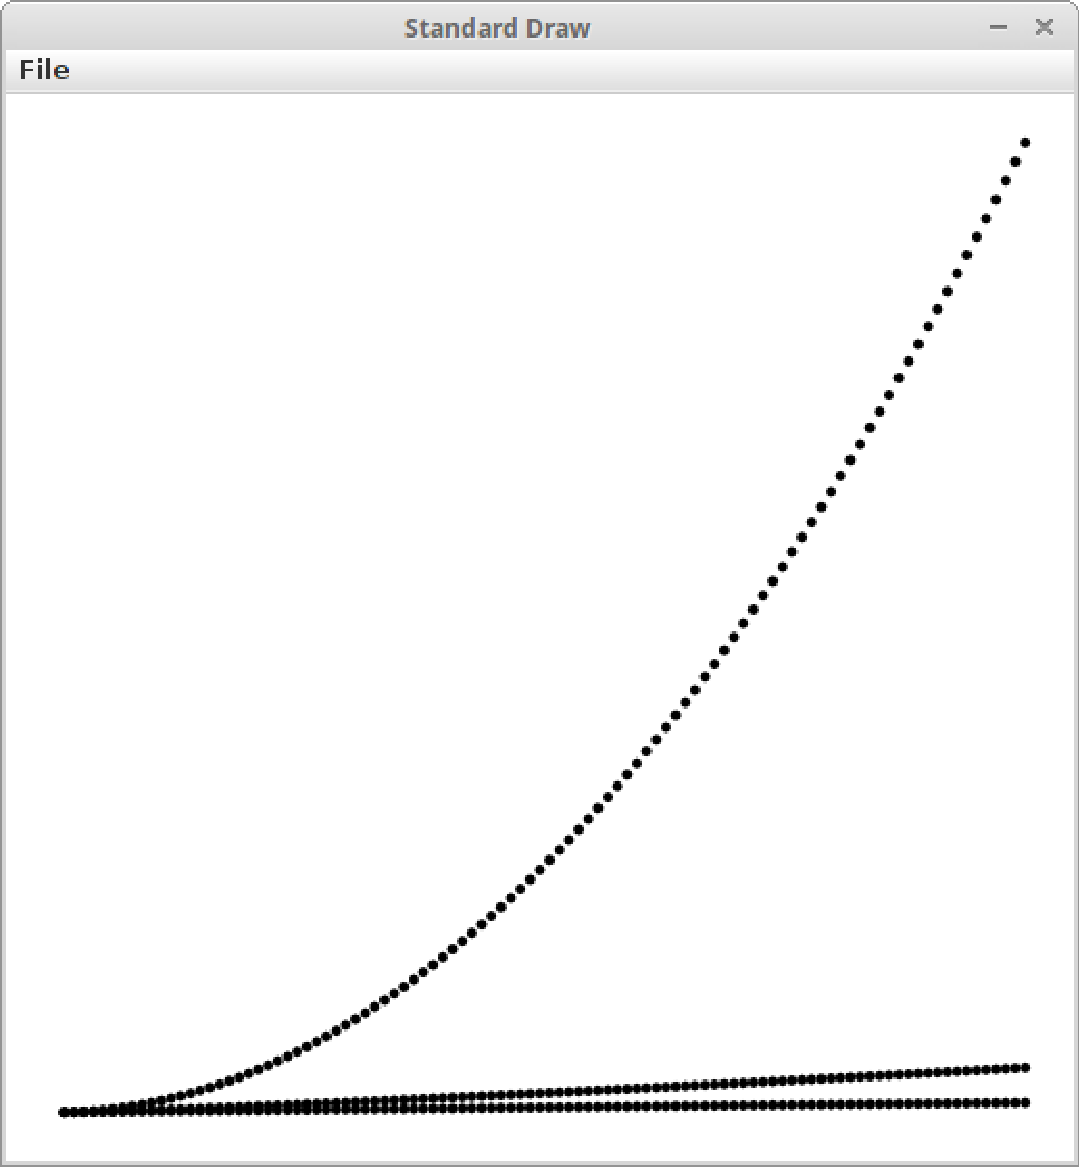
\includegraphics[scale=0.25]{./figures/functions.pdf}
\end{minipage}
\end{itemize}
\end{frame}
\end{document}
